\documentclass[11pt,a4paper,english]{article}
\usepackage[T1]{fontenc}
\usepackage[utf8]{inputenc}
\usepackage[english]{babel}
\usepackage[a4paper]{geometry}
\geometry{verbose}
\usepackage[authoryear,round]{natbib}
\usepackage{color,graphicx}
\usepackage{amsmath}
\usepackage[unicode=true,
	colorlinks=false,
	backref=false,
	linkbordercolor={1 1 1},
	urlbordercolor={1 1 1},
	citebordercolor={1 1 1}]{hyperref}
\hypersetup{
	pdftitle={On Statistical Metrics for Selection and Phrasality},
	pdfauthor={Damir Ćavar},
	pdfsubject={Syntax and Statistics},
	pdfkeywords={Mutual Information, Relative Entropy, Parsing}
}
\usepackage{linguex}
\usepackage{qtree}
\usepackage{float}
% line spacing
\linespread{1.5}


\title{On Statistical Metrics for Selection and Phrasality\footnote{This paper is based on so far unpublished joint work with my former research assistants and students Paul Rodrigues and Giancarlo Schrementi in the Computational Linguistics Lab at Indiana University (IU). They had a significant contribution to this project. We are all grateful to IU and IU's Linguistics Department for making this work possible. However, I am most grateful to Peter Staudacher for his inspiring comments on all the linguistic topics we discussed, not dismissing even the most devious ideas and analyzes I came up with. It was, and always is a pleasure to have him around, not just because of his profound knowledge, his social consciousness and well-grounded political views, but also because of his distinct sociability and constancy.}}
\author{Damir Ćavar\\ Linguistics Department\\ University of Zadar}
\date{February 2010} 


\begin{document}

\maketitle


\section{Introduction}

In the following we shall discuss a fairly simple empiricist approach to syntactic structure, which could be considered as some sort of exemplar model.\footnote{Here we consider recent research discussed and described in \cite{Bod:2009} and related work, as the relevant type of exemplar model that we relate to here.} We compare this approach and its empirical results and theoretical consequences briefly with a common qualitative theory that is utilizing symbols and rules. The research goal is to evaluate the usability of various information theoretic metrics for unsupervised syntactic chunking, and potentially even basic parsing.

The presented experiment is based on ideas formulated in \cite{Magerman:Marcus:1990}, and \cite{Magerman:1994} where Mutual Information (MI) over Part-of-Speech tags in annotated corpora is used as a metric for the identification of syntactic \textit{attraction} or simply phrasality. A more detailed discussion of this method is presented in section \ref{Sec:MagermanMI}.

We compare the results of the MI-based approach with results from alternative measures using the same strategy for identification of phrasality. The identification of syntactic phrases or chunks in the second approach is performed by relating pruning decisions to Relative Entropy (RE) scores for adjacent tokens. As mentioned in \cite{Cavar:ea:2004}, this measure might be more adequate given its directional nature (RE) and the relevant properties of syntactic relations.

Our experiments describe the results of grouping lexical items into phrase-like units in raw text. We use an incremental learning algorithm, i.e.\ one that learns and applies the syntactic chunking of raw text in parallel, as described in \cite{Cavar:ea:2004}. This way we have access to the learning curve, and we can track the development of the statistical n-gram model, as well as the results of its application on the input data.

Although the syntactic phrasing and chunking results in the discussed experiments are moderate, they seem to show that such an incremental unsupervised learner/parser converges to a stable performance, reaching a constant plateau, without tendencies to break out with longer learning/parsing time. Finally, the implications of methods and results have some relevance for theoretical syntax, as discussed in section \ref{Sec:Conclusions}.



\section{Previous work}\label{Sec:MagermanMI}

There are numerous research projects and results available in the domain of statistical parsing using for example a metric based on concepts from Information Theory \citep{Shannon:1948}. Unfortunately, we cannot discuss them all here. Instead we concentrate on the core ideas and reported results from a paper published by \cite{Magerman:Marcus:1990}, and related to e.g.\ \cite{Church:1988}.

\cite{Magerman:Marcus:1990} suggested an algorithm for constituent recognition or simplified parsing using MI scores over Part-of-Speech (PoS) tags from an annotated corpus. They base their study on the Brown corpus \citep{Francis:Kucera:1982} with a reduced subset of 64 PoS-tags. Given a sequence of tokens, the suggested structure assigning algorithm determined a non-constituent (`distituent', as described below) excited at the point in the given sequence where MI was at a local minimum. At this point, a syntactic boundary was spliced in. Each sequence is thus split into two sub-constituents, and each resulting constituent with more than two token is recursively split using the same approach.

The MI score determines the amount of information shared between two items. In this approach it is based on unigram and bigram statistics of PoS-tags. \cite{Magerman:Marcus:1990} suggest it to be calculated using the following equation:

\begin{equation}
MI(x,y)=log\frac{P(x,y)}{P(x)P(y)}
\end{equation}

Here the probability $P(x,y)$ is the observed maximum likelihood of the bigram containing the tokens $x$ and $y$, i.e.\ it is the relative frequency of the bigram $xy$ calculated on the basis of a given corpus. Similarly, the probabilities $P(x)$ and $P(y)$ are unigram probabilities of the single tokens, i.e.\ relative token frequencies, ideally taken from the same corpus as the bigram frequencies.

Besides the common interpretation from Information Theory \citep{MacKay:2003}, there are alternative interpretations of the MI metric. One possible interpretation of the MI formula above could be, in the sense of hypothesis testing, that it looks at the ratio between two probability distributions, the observation and the expectation of two events co-occurring. The expectation (given some null-hypothesis) could be that the two variables $x$ and $y$ are independent, i.e.\ the likelihood of $x$ and $y$ co-occurring should be the product of their individual occurrence likelihoods. If the two variables are independent, the observed and the expected likelihoods should be close or ideally equal to each other. Thus the ratio should be close to $1$, and consequently the logarithm close to $0$.\footnote{We assume the logarithm to the base of $2$ here.} Thus, if two variables are rather independent, the resulting MI score will be low, approaching $0$. The higher the mismatch between the observation $P(XY)$ and the expectation $P(X)P(Y)$, the higher the resulting MI score. In other words, the more likely the two variables $x$ and $y$ are dependent, the larger the ratio between observed and expected likelihood, the larger the resulting MI score.

From an empirical perspective, one might expect that the MI score for a sequence of PoS-tokens \textit{Article Noun} is much higher then for example for a sequence \textit{Noun Verb}, given that in ca.\ 80\% of the cases an article is followed by a noun in any common English text corpus, while the observed probability of a noun being followed by a verb is significantly smaller.

In particular, \cite{Magerman:Marcus:1990} calculate the MI score over unigrams and bigrams of PoS-tags, and not word or string tokens, i.e.\ they use statistical models from linguistically annotated data. In fact, \cite{Magerman:Marcus:1990} suggest the more general weighted metric Generalized Mutual Information (GMI), which can be applied to any token window size, and is calculated using bigram statistics.

\begin{equation}
GMI_{i+j}(x_1 \dots{} x_i,y_1 \dots{} y_j)=\sum_{\footnotesize\begin{array}{c}
X \mbox{ ends with } x_i\\
Y \mbox{ begins with } y_1
\end{array}} \frac{1}{\delta{}XY} MI(X,Y) 
\end{equation}

This formula calculates the GMI score for all token pairs as the sum of the MI scores of all ngrams in which the first token is the right-peripheral element of the initial ngram, and the second token is the left-peripheral element of the second ngram. This score is weighted with the reciprocal of the standard deviation $\frac{1}{\delta{}XY}$ of the MI score of one such token pair over the complete distribution.

The statistical models are generated by moving a window of two tokens along a token sequence of a sentence taken from the corpus. The suggested algorithm in fact pads each sentence on both sides with empty tags, up to the maximum word window size (minus 1), thus, as the authors point out, normalizing the sentence lengths and creating the adequate context for GMI calculations.

By searching the local MI minimum in a sentence, \cite{Magerman:Marcus:1990} try to identify so called \textit{distituents}, i.e.\ adjacent PoS-tokens that are unlikely to be adjacent within a syntactic constituent. In other words, local MI minima in a token sequence intuitively seem to correspond to a situation where one token does not contribute a lot about its neighboring token. This is what we expect to find when a PoS-tag to the respective side does not restrict the choice of PoS-tokens due to the lack of syntactic category or semantic selection. We will come back to this in the following section.

In addition to the statistical constituent boundary metric, \cite{Magerman:Marcus:1990} include a dictionary of predefined distituents as a supervision component in their otherwise mostly unsupervised statistical distituent parsing algorithm. In the following examples, such distituents assign the MI score of $-\infty$ to corresponding PoS-sequences. One such distituent is for example the sequence \textit{noun preposition} in example \ref{Ex:ParseMIDGPass} below. The logic of overriding the real MI score is related to the fact that higher MI scores indicate higher probability of two items belonging to one constituent. A sequence of \textit{noun preposition} in the selected corpus is frequent enough, such that it would wrongly suggest a head noun and a right adjacent preposition to be part of one basic syntactic constituent. Assigning $-\infty$ scores to hand-crafted distituents indicates no probability at all for two adjacent items to be syntactically related in terms of sister nodes (or maybe head and complement).

The parser recursively recognizes distituents over a sequence. For the example in \ref{Ex:ParseMI} \cite[][pg.\ 987]{Magerman:Marcus:1990}, the initial pass generates the GMI scores for all PoS-bigrams.

\exg. {\small\textit{He} ~ \textit{directed} ~ \textit{the} ~ \textit{cortege} ~ \textit{of} ~ \textit{autos} ~ \textit{to} ~ \textit{the} ~ \textit{dunes} ~ \textit{near} ~ \textit{Santa Monica.}}\\
      {\small pro 3.28 verb 3.13 det 11.18 noun 11.14 prep 1.20 noun 7.41 prep 16.89 det 16.43 noun 12.73 prep 7.36 noun}\\\label{Ex:ParseMI}

The handcrafted distituent grammar assigns maximally low scores to bigram distituents, as in \ref{Ex:ParseMIDGPass}, resulting in a first chunk sequence as in \ref{Ex:ParseMIAfterDG}.

\ex.\label{Ex:ParseMIDGPass} pro 3.28 verb 3.13 det 11.18 noun $-\infty$ prep 1.20 noun $-\infty$ prep 16.89 det 16.43 noun $-\infty$ prep 7.36 noun

\ex.\label{Ex:ParseMIAfterDG} {[ he ] [ directed ] [ the cortege ] [ of autos ] [ to ] [ the dunes ] [ near Santa Monica ]}

According to \citet[pg.\ 987]{Magerman:Marcus:1990}, a threshold will prevent close scores from being considered significantly different. Thus 3.28 and 3.13 are considered local minima, and thus the respective bigrams are assumed to be distituents. The resulting structure after the third pass is illustrated in \ref{Ex:ParseMIFinal}. The algorithm stops when no further distituent can be identified.

\ex.\label{Ex:ParseMIFinal} [ he ] [ directed [ [ the cortege ] [ of autos ] ] ]  [ [ to [ the dunes ] ]  [ near Santa Monica ] ]

Without offering relevant details, \cite{Magerman:Marcus:1990} report good results at parsing short sentences. An average error rate of one error per sentence for short input sentences was reported. The average error rate increased to two errors per sentence in sentences with conjunctions. In long sentences with a length between 16 and 30 words, the average error rate was reported as 5 to 6 errors. Unfortunately, there is no detailed information available about the error types in all the different cases.

It is important to note, however, that these results were achieved with supervision. They included a hand-crafted distituent list in their parsing algorithm. This list would enforce PoS-sequences of the type \textit{Noun Preposition} to be excluded as an adjacent sequence within constituents. Some such sequences might in fact be assigned a higher MI score.



\section{Resulting questions and issues}

The discussed algorithm has various interesting properties. It generates hierarchical structures in a bottom-up fashion, and the generated structures are n-ary-branching trees. In fact, it seems to be purely statistically driven.

However, it is obvious that there are a couple of crucial conditions and supervision steps included in the algorithm. As already mentioned, handcrafted distituent grammars are obviously essential, otherwise we could expect the performance of the algorithm to drop dramatically, as the example above illustrates.

It is also important to note that the statistical models are extracted from linguistically annotated corpora, i.e.\ the supervision enters the statistical models via preprocessed language data and classification information as PoS-tags.

Additionally, the integration of arbitrary thresholds, and other manually fixed values that are not discussed in this short description here, classify it for a supervised algorithm.

It might be that the achieved results in fact dramatically depend on these supervision means, i.e.\ that they are real side-effects of intelligent design and supervision, rather than emerge from statistical and distributional properties of language as such. If so, it would be impossible to draw any theoretically relevant conclusion from these experiments about properties of English or language in general, or other consequences for the assumption about for example learnability.

Furthermore, the presented models are generated as static models in a training phase, using a complete corpus, or a large portion of it.\footnote{A common strategy is that portion of the corpus is not used for generation of the respective statistical models. The same strategy was used by \cite{Magerman:Marcus:1990} in the discussed experiments.} It is not clear, how this approach would perform on other genres and languages. To be more precise, our research hypotheses include the specific hypothesis that a learner is equipped with dynamic memory (or a dynamic language model), which adapts to the input, and at the same time is applied to it, processing the input it learns from. Static statistical models are not necessarily appropriate for our own research goals and experiments, which are related  learnability and psycholinguistic and theoretical issues of knowledge of language.

Another theoretical question is related to the nature and purpose of syntactic trees. Some syntactic theories might not necessarily aim at representing hierarchical relations in a semantically relevant way. In the generative tradition, structural syntactic relations are associated to semantic scope relations, i.e.\ the interpretation of a sentence is associated with its syntactic structure. Scope is not necessarily a concept in dependency trees, though. The question thus is, whether such scope relations can be identified systematically, with such statistical approaches, and to what extend scope errors might occur in the resulting trees.

With respect to the distituent or constituent metric, MI is not necessarily the optimal choice for describing and evaluating potential syntactic relations. One reason is that syntactic relations are typically unidirectional, which is also part of the nature of hierarchical relations. Usually just one lexical item or category requires or selects another category or syntactic structure, while the latter usually does not restrict the former, at least not in the same way. To exemplify this, consider the minimal pair in \ref{Ex:CSel1a}--\ref{Ex:CSel1b}:

\ex. \textit{John saw a bird.}\label{Ex:CSel1a}

\ex. *\textit{John saw in Paris.}\label{Ex:CSel1b}

The ungrammaticality of \ref{Ex:CSel1b} in generative grammar might be attributed to a violation of lexically specified selectional properties of verbs \citep[e.g.][]{Chomsky:1965}. In this particular example, a valid assumption might be taht the verb \textit{to see} requires its direct object to be a noun phrase, as in \ref{Ex:CSel1a}, rather than a preposition phrase as in \ref{Ex:CSel1b}. On the other hand, it would be difficult to state something similar for the noun phrase \textit{a bird} or the preposition phrase \textit{in Paris} in the examples above.

If we extend this concept of restrictive relation or selection to the lexical level, we might come to similar conclusions. The occurrence of the article \textit{the} makes native speakers of English expect a noun to appear in the immediate local context, following the article. They would probably not have a clear intuition about some concrete noun to follow, i.e.\ they tend to have categorial intuitions associated with concrete lexical forms. On the other hand, our intuition about the preceding context of \textit{the} seems to be rather deficient. We can test this for example in cases where the preceding word was rendered incomprehensible using noise.

In fact, as with the examples \ref{Ex:CSel1a}--\ref{Ex:CSel1b}, the occurrence of the article \textit{the} triggers the expectation of a specific syntactic category to follow it. However, with other lexical elements it might be that the expected property in the immediate right context is that of a concrete lexical element. For example, prepositions or certain verbs seem to have a more lexical association. The co-occurrence frequency of a preposition and an article might be responsible for the strong association between for example \textit{on} and \textit{the} to the right of it, or similarly for the sequence \textit{said} and \textit{that}. Here too, the occurrence of \textit{the} does not seem to let native speakers of English expect a \textit{on} to precede it. Neither does the occurrence of \textit{that} increase significantly the expectation of a preceding \textit{said} in its immediate context.

While it seems obvious that syntactic relations and lexical selections or dependencies are directional, the MI metric on the other hand is not.

MI relates the probability of two events co-occurring $P(XY)$ to the probability of them co-occurring and not being dependent on each other $P(X)P(Y)$. As for the logical AND operator, it is in principle irrelevant in which order $X$ and $Y$ co-occur. We might expect a non-directional metric like MI to be less relevant for syntactic relations, where directionality seems to play a role. Additionally, one of the problems of the presented approach is also that the trees are not labeled, and it is not trivial to discriminate automatically the head from its complement in the resulting structures. The authors are vague about this issue, and indeed imply specific hierarchical relations in their example parse, which are not as obvious, or in fact, seem to be geared towards an ideal parse.\footnote{The presented structural representation implies a hierarchical head-complement relation as in $[$ \textit{to} $[$ \textit{the dunes} $] ]$ while the parse history suggests a non-hierarchical structure with \textit{sister} relations, as $[ [$ \textit{to} $] [$ \textit{the dunes} $] ]$.}

Furthermore, MI is a frequency sensitive score. The lower the frequency of the relevant tokens, the more unreliable MI is. This can be easily verified with some simple examples of low-frequent tokens co-occurring in corpora. However, in an approach as presented in \cite{Magerman:Marcus:1990}, this does not seem to be relevant, since the chosen strategy was to use PoS-tags for statistical ngram models, and not words. Additionally, the authors also use a reduced set of PoS-tags, boosting their distributional statistics even more, and thus MI is in fact expected to be more reliable.

\cite{Magerman:Marcus:1990} emphasized that on the word level the described approach would require much larger corpora to overcome the data scarcity problem. However, it is not clear how big the differences between the word- and the PoS-tag level really are, given the proposed information theoretic statistical metrics and measures. It would be interesting to see how much of the `dominant syntactic properties' potentially correlates with statistical and distributional properties intra- and cross-linguistically. Furthermore, from an empirical and data driven perspective, it would be useful to establish a hierarchy of necessary supervision strategies that could guide such algorithms either as language specific strategies, or maybe even cross-linguistic ones.


\section{Experimental strategies and evaluation}

In the following we shall lay out the goals and concepts of our experiments, which are based on the ideas and resulting questions and critiques of \cite{Magerman:Marcus:1990}, but focusing on the following design strategies:

\begin{itemize}
\item Incremental learning algorithms
\item Dynamic statistical models
\item Minimization of supervision strategies
\end{itemize}

Our focus on incremental learning algorithms and dynamic statistical models is related to general research hypotheses and questions of learnability and convergence of models. In our implementation of a statistical parser and learner, every input sentence is immediately extending the statistical language model, and the parser generates with every input sentence a hypothesis about its structure.

The language models that we use, are unigram and bigram models, similar to the parser discussed above. As input we use raw word tokens and PoS-tags from a portion of the Penn Treebank \citep{Marcus:ea:1993}. From the word tokens and PoS-tags we generate four types of models, including mixed models that use word tokens and PoS-tags.

\begin{itemize}
\item token -- token
\item token -- type
\item type -- token
\item type -- type
\end{itemize}

The reason for testing all these mixed models is related to the mentioned intuition that prediction and expectation of token and type correlations and co-occurrences seem to be part of the cognitive ability of native speakers. By testing comparatively the token--token and type--type models, we can also directly evaluate the predictions that are common in the literature that token--token relations are problematic because of the data scarcity problem.

Our suggested parsing method is much simpler than the method suggested by \cite{Marcus:ea:1993}. We use two metrices for the evaluation of distituents or constituents, MI and Relative Entropy (RE) or Kullback–Leibler divergence. MI is calculated for each bigram $<\!xy\!>$ and the respective unigrams in the following way \citep[cf.][]{MacKay:2003}:

\begin{equation}
P(<\!xy\!>\!|x) ~ lg \frac{P(<\!xy\!>)}{P(x)P(y)}
\end{equation}

That is, we take into account only directional probabilities, by only considering bigram probabilities of bigrams where $x$ occurs only as the left or initial item in a bigram.

RE is a comparison or distance measure of two probability distributions. We compare the likelihood of $y$ occurring independently, with the likelihood that it occurs, given that $x$ occurred. If $x$ and $y$ are statistically independent, then $P(y|x)$ should be equal to $P(y)$. If the two variables are dependent, $P(y)$ is smaller than $P(y|x)$, than the resulting RE-score will be low, potentially even negative. It is calculated for each bi-gram $<\!xy\!>$ in the following way:

\begin{equation}\label{Eq:RelativeEntropy}
P(y) ~ lg \frac{P(y)}{P(y|x)}
\end{equation}

Given the specific architecture that we want to test here, and for simplicity reasons, zero probabilities of previously unseen tokens and bigrams do not occur, i.e.\ if an item is in the input sentence, it is immediately integrated into the statistical language model. This happens before the respective model with the previously unseen events is applied to parse the respective input.

An alternative strategy one might pursue could be to treat items differently that have not occurred before, by using the string entropy as the RE-score, as given in the following formula:

\begin{equation}
lg~26 \cdot len(y)
\end{equation}

Here we assumed the number of different characters in the respective corpus, text, or language to be 26. Furthermore, for simplification reasons we assume that the likelihood of every character to occur is equal. The entropy of the string is then the product of the number of characters in the string (word token in our case) and the logarithm to the base of two of the number of characters. It did not seem relevant for our purpose here to provide more detailed estimates of the entropy of a previously unseen string.

Even more advanced strategies might include various smoothing techniques to cope with unseen data from the training corpus. Once again, the model we test here makes no distinction between training and test corpus. It is an incremental learner model.

The difference between RE and MI becomes clear, if the respective equations above are compared. RE is an asymmetric measure, i.e.\ the RE score should differ for two different items $x$ and $y$ occurring in the same bigram, if their individual probabilities differ.

As already mentioned, RE also behaves differently then MI, i.e.\ the lower the RE-score, the higher the probability that two distributions are related, in a directional sense. We expect RE to be better suited for directional selection effects, as we can find them in syntax.

The differences between MI and RE, and in particular the fact that RE seems to be better suited for specific lexical induction tasks was pointed out in \cite{Lee:1997}. The superiority of RE for measuring and predicting certain linguistic relations has been confirmed also in a morphological segmentation task as described in \cite{Cavar:ea:2004b}.

The algorithm that we use is similar to the already discussed one, i.e.\ we introduce phrase boundaries where the MI-score is lowest, or the RE-score is highest. However, in principle, there are various potential strategies to parse the input sequence, and we are interested in the differences between them, with respect to the model we choose. The top-down strategy could identify the absolute MI minimum or RE maximum, and split the sequence of items there, and continue recursively splitting the individual chunks, as long as there are more than two items left in each of them. Alternatively, the bottom-up strategy could combine two items or chunks (or any other combination of chunks and items) into one chunk, whenever between such items the  MI-score is highest or the RE-score is lowest within its domain (sentence or chunk). The following example illustrates a top-down pruning strategy, and the resulting tree, using the example \ref{Ex:ParseMIDC} from above.

\exg. {\small\textit{He} ~ \textit{directed} ~ \textit{the} ~ \textit{cortege} ~ \textit{of} ~ \textit{autos} ~ \textit{to} ~ \textit{the} ~ \textit{dunes} ~ \textit{near} ~ \textit{Santa Monica.}}\\
      {\small pro 3.28 verb 3.13 det 11.18 noun 11.14 prep 1.20 noun 7.41 prep 16.89 det 16.43 noun 12.73 prep 7.36 noun}\\\label{Ex:ParseMIDC}

Using the distituent-strategy, the sequence in \ref{Ex:ParseMIDC} would be recursively split into two segments, where within the segment the lowest MI score occurs. This would be applied to all resulting sequences (potential constituents), until a further segmentation is impossible. In the initial segmentation step applied to the PoS-tags the resulting two segments are displayed in \ref{Ex:ParseMIDCa}. The subsequent segmentation step leads to the structure in \ref{Ex:ParseMIDCb}.

\ex. [ {\small pro 3.28 verb 3.13 det 11.18 noun 11.14 prep} ] [ {\small noun 7.41 prep 16.89 det 16.43 noun 12.73 prep 7.36 noun} ]\label{Ex:ParseMIDCa}

\ex. [ [ {\small pro 3.28 verb} ] [ {\small det 11.18 noun 11.14 prep} ] ] [ [ {\small noun 7.41 prep 16.89 det 16.43 noun 12.73 prep} ] [ {\small noun} ] ]\label{Ex:ParseMIDCb}

The final tree structure for the given example using the top-down MI-minimum pruning strategy based on PoS-tag unigram and bigram statistics is illustrated in \ref{Ex:ParseMIDCTree}.

\ex.\label{Ex:ParseMIDCTree} {\footnotesize\Tree[ [ [ he directed ]  [ [ the cortege ] [ of ] ] ]   [ [ [ autos ] [ [ [ to the ] [ dunes ] ] [ near ] ] ]  [ Santa~Monica ] ] ]}

And, in fact, the same structure would result, if we apply a bottom-up constituency approach based on the PoS-tag statistics. In a constituency approach we would merge two adjacent tokens into one constituent, where we reach a local MI-maximum, recursing over the complete sequence. The resulting tree for the given example using such an approach should correspond to the one in \ref{Ex:ParseMIDCTree}.

However, we do expect different tree structures to result from using the RE-score, or even other statistical models and measures. As already mentioned, we could consider the MI and RE scores based on any of the four combinations of elements in a bigram, i.e.\ token--token, token--type, type--token, and type--type.

%\ex.\label{Ex:ParseMIDCTreeB} {\footnotesize\Tree[ [ [ he directed ] [ [ the cortege ] of ] ] [ [ autos [ [ [ to the ] dunes ] near ] ] Santa~Monica ] ]}

It is obvious that the resulting tree in \ref{Ex:ParseMIDCTree} would not pass the professional rating of syntacticians. It is definitely not an accurate syntactic representation of the underlying sentence. However, parts of it might be. Our research question is to find out to what extend it could be possible to recognize phrases and structural properties using just the simplest baseline strategies.

Using these strategies, the resulting trees would always be strictly binary branching. However, the trees do not provide constituent labels. It would not be obvious to decide which of the tokens in a constituent could be the head. We do not deviate here from the parsing strategy discussed above.

On the other hand, if the feature-make-up of the tokens would be available in the resulting tree, the category properties could be handled lexically, in a similar way as suggested for example in the Minimalist Program \citep{Chomsky:1995} or variants of lexically driven grammars, like for example categorial grammars \citep[e.g.][]{Steedman:2001}.

We expect the RE-score, since it is directional, to provide a clue about the potential head-position in the sense that one element in the constituent will be statistically more restrictive towards one side. With statistical restrictiveness we mean that the variation of the number of different tokens or PoS-tags might be smaller on one side, then on the other. This could be interpreted as some sort of selection, either c(ategory)- or s(emantic)-selection.


The MI-score is used in the following way. For every input sentence and for every bigram in the sentence the MI value is calculated. The sentence is split into two parts at the lowest MI-value, and this is repeated recursively for every resulting part, up to the token level. Each split introduces two new constituents in syntactic terms. For each bigram type (token--token, token--type, type--token, type--type) using the MI-score one syntactic structure is generated.

The RE-score is used in the same way, splitting the sentence at the maximum RE-score of one of the contained bigrams, and recursively applying this splitting operation to the resulting sub/constituents, as in the case of MI-based sentence segmentation.

The parser outputs eight different sentence structures that are annotated with a score that represents the evaluation score, which is determined by comparing the Penn Treebank structure with the generated structure (matching and mismatching brackets). The score is the total of the distance between the left and right parentheses distances.

The architecture of the system allows for offline training as well as dynamic online training. Included are functions that extend the language model with every input sentence, i.e.\ the token and bigram statistics are updated and persistently stored. Thus, with every evaluation phase the language model is incrementally trained or extended. This provides insights into the runtime development of the languages model, its development curve and accuracy for all parameters (i.e.\ the statistical scores MI and RE, as well as the token or type information used).


\subsection{Training and testing corpora}

The parser was trained and tested using the Brown corpus \citep{Francis:Kucera:1982} with a reduced PoS-tag set. All punctuations were left unchanged. The lexical PoS-tags were reduced to 11 basic lexical classes, e.g.\ verb, noun, preposition etc.

The evaluation is based on the data in the Penn Treebank \citep{Marcus:ea:1993}, i.e.\ the same data used in \cite{Magerman:Marcus:1990}.\footnote{The initial test was performed on 10\% of the Penn Treebank. A test sample is for example provided in the data package of the Python Natural Language Toolkit \citep{Bird:ea:2009}.} The advantage of using the sentences from the Penn Treebank are that the sentence structure is provided and can be used for immediate runtime evaluation. In our implementation of the experiment the parser consumes raw sentences as either sequences of word tokens, PoS-tags, or a combination of both. The evaluation of the resulting parse tree is automatically performed by comparing the bracketing provided in the corpus with the hypotheses generated by the parser.

Given the fact that trees in the Penn Treebank are not strictly binary branching trees, the evaluation scores are to be taken as tendencies. A detailed analysis of the resulting parser accuracy would still require manual evaluation and judgment.


\section{Results}

The preliminary results indicate that type--type relations result in structures that better match the Penn Treebank trees. Once again, the Penn Treebank does not contain purely binary branching trees. A mismatch is expected and the resulting evaluation cannot make direct quantitative statements about parsing accuracy.

On the tests performed so far, the RE-based segmentation is outperforming the MI-based segmentation, however, not by a large margin.

The results based on one experiment using the Brown corpus as a training set, and 10 \% of the Penn Treebank as the evaluation basis are illustrated in the time plot in figure \ref{Fig:ParseAcc}. The lower the score in this plot, the better the parse tree in comparison to the Penn Treebank trees.

\begin{figure}[h]
\centering
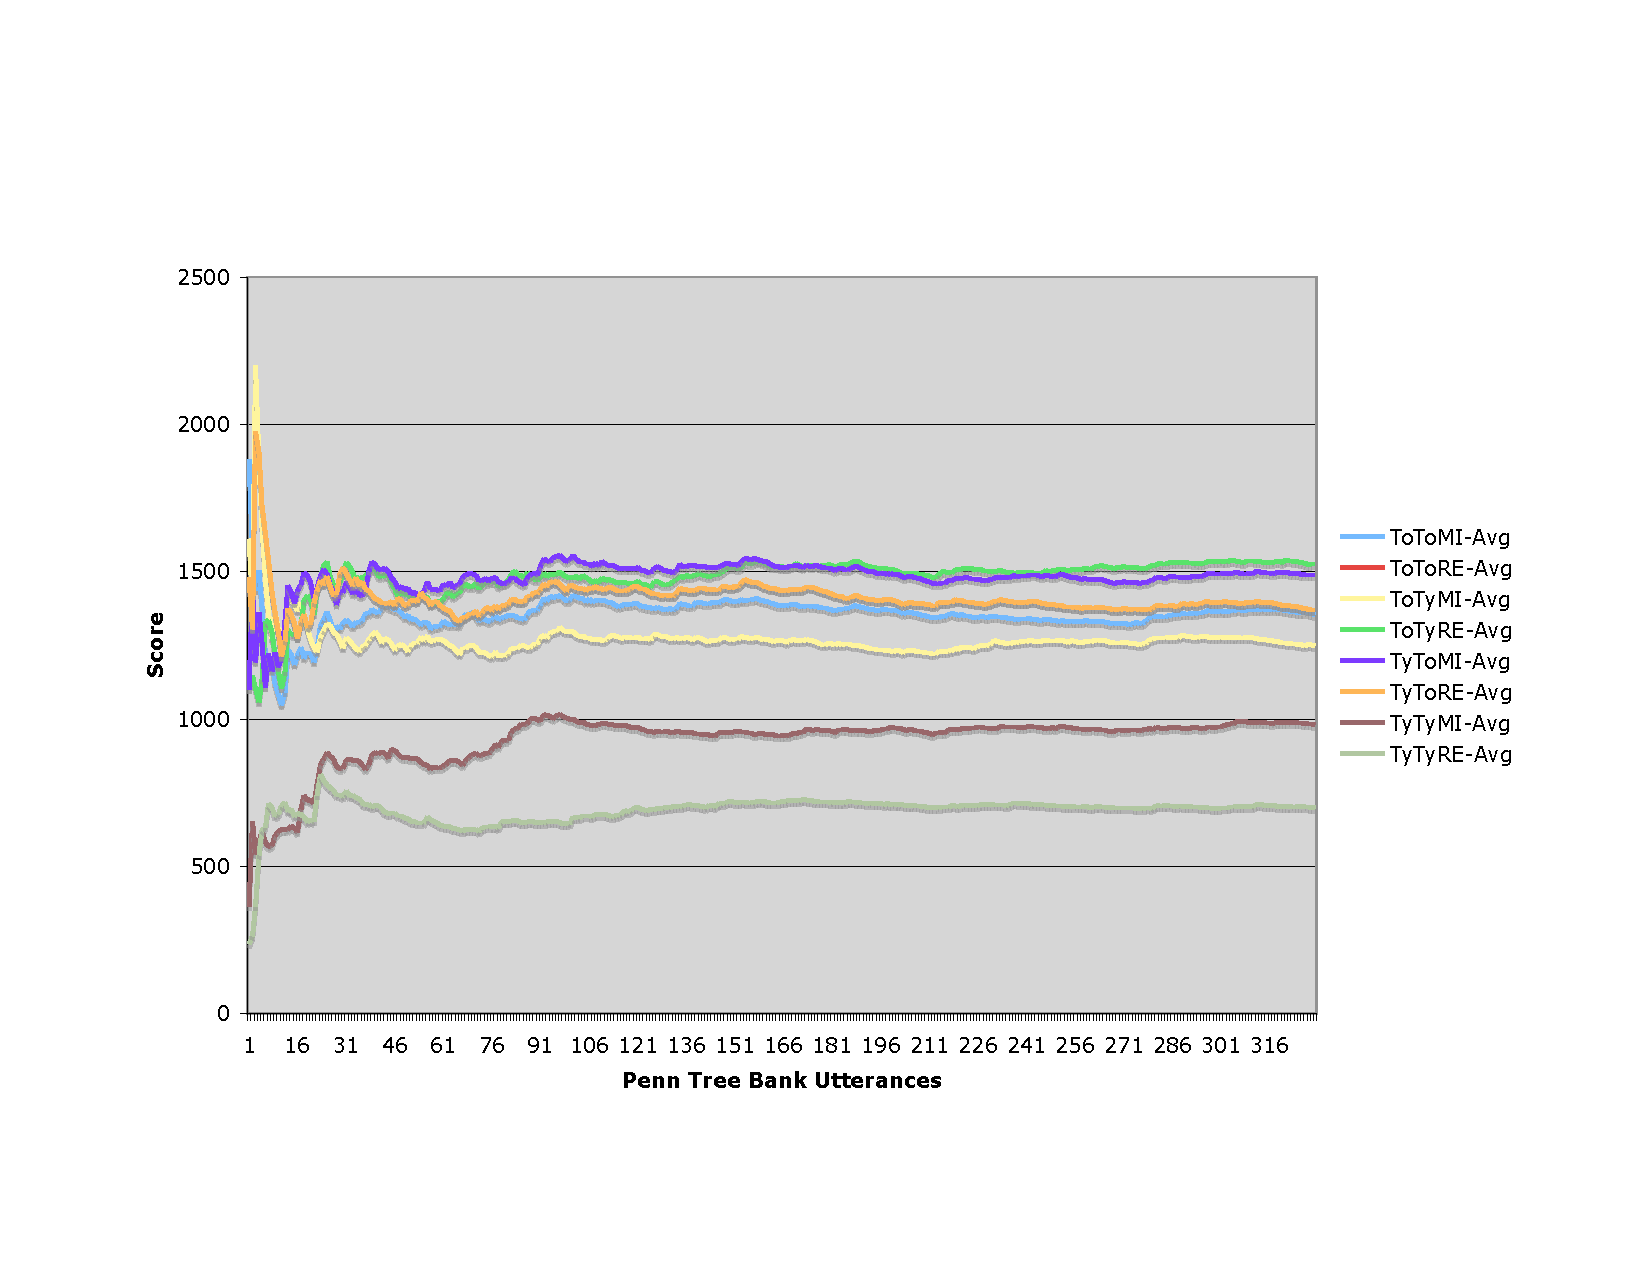
\includegraphics[scale=0.55]{mip-cut-results.pdf}
\caption{\emph{Parsing accuracy over time}\label{Fig:ParseAcc}}
\end{figure}


\section{Conclusion}\label{Sec:Conclusions}

We can conclude that for a syntactic parse type--type relations give better results than any token-based relation. This was expected. Both type--type parse strategies are clearly better than any of the other models. In fact the type-statistical models are much more dense than the pure word token statistics.

The reduction of the PoS-tags in the Brown corpus boost the statistical models, but it could in fact introduce new problems. We have not tested for the effect of the PoS-tagset reduction. The tests on the full Brown tagset have not yet been performed.

The fact that the RE-based segmentation outperforms the MI-based ones, could be interpreted as being due to the fact that syntactic relations indeed are asymmetric. This is one of the expected results.

There is a lower token--token accuracy, which might be due to independent effects of token frequencies and their common distribution properties. We tested the token \textit{the} for example for its average MI- and RE-score to the left and right. This can be done by averaging the sum of all MI-scores for bigrams in which the token \textit{the} occurs in second position, and taking this score to be the left average MI-score of \textit{the}. Calculating the same score for all bigrams in which the token \textit{the} occurs in the initial position would be the right average MI-score for it. If we compare this also with the corresponding average RE-scores left and right of \textit{the}, we can see that in the Brown corpus the left MI-score for \textit{the} is higher than the right one.


This could mean that the variation of tokens to the left of \textit{the} is much lower than to its right. This is counterintuitive, as already discussed in the previous sections. Overall, our expectation is that the right context of \textit{the} is much more restricted. But, given the fact that \textit{the} occurs frequently in sentence initial position, and less frequently, or not at all in sentence final position, artificially creates this distributional statistical property.

One way to improve the statistics of elements that tend to appear frequently in sentence initial or sentence final position would be to pad every sentence with a randomly generated non-word token left and right, as shown in example \ref{Ex:PaddedS}.

\ex.\label{Ex:PaddedS} \texttt{26376182 The answer is a new era . 78655465}

The bigram model will then include many bigrams with \textit{the} preceded by some random number, but the frequent occurrence of it in sentence initial position with its artificial effect of variation reduction would be neutralized. In fact, the properties of most of the highly frequent function words would actually correspond to their syntactic properties, i.e.\ being selective towards one side, as illustrated in table \ref{Tbl:AVREMI}.

\begin{table}[H]
\centering
  \begin{tabular}{ccccccc}
  \textbf{Av.L.RE} & \textbf{token} & \textbf{Av.R.RE} & ~~~~ & \textbf{Av.L.MI} & \textbf{token} & \textbf{Av.R.MI} \\\hline
  +              & \textit{the}   & -- & & -- & \textit{the} & + \\
  +              & \textit{a}   & -- & & -- & \textit{a} & + \\
  +              & \textit{on}   & -- & & -- & \textit{on} & + \\
  \end{tabular}
  \caption{\emph{Average left and right RE and MI for single tokens}\label{Tbl:AVREMI}}
\end{table}

The average left and right RE and MI scores for highly frequent function words o indeed provide accurate structural information. In fact, they could be used as cues for the induction of selection directions and headedness in phrasal structures. In our parsing algorithm the introduction of constituent boundaries at high RE and low MI scores at one side of such prominent function words would dramatically improve the parse accuracy.

Given the presented baseline results, it seems to be clear that:

\begin{itemize}
\item Statistical properties of the distribution of tokens or PoS-speech tags can be used for the induction of syntactic properties. Maybe even structural selection or restriction properties of some tokens can be induced, and consequently for example headedness, transitivity etc.

\item Dynamic n-gram, as described in this particular task, seem to stay robust with respect to their accuracy, independent of the size of the training corpus. Incremental learning seems to converge to some stable plateau.\footnote{This needs further detailed testing with much larger corpora.}
\end{itemize}

In future experiments the observations and expectations need to be tested on other languages, with much larger corpora. The role of the PoS-information, whether it is more general, or specific and detailed, should be evaluated as well.

In general, what these type of experiments seem to show is that statistical distributional information about linguistic units in specific linguistic contexts can reveal some significant portion of structural information. Here one has to be careful with conclusions about empirical versus deductive theoretical models. As has been shown, the statistical models that take discrete linguistic information into account outperform purely empirical ones (i.e.\ word token based models).

The implementation of the described parser in Python, the relevant data, and the log files and further information packages used in these experiments are available under the Creative Commons license at the following URL:\\
\url{http://ling.unizd.hr/~dcavar/MIREParse/}


\bibliographystyle{plainnat}
\bibliography{main}

\end{document}
\end
